\section{Application: Systems of linear differential equations}

\begin{outcome}
  \begin{enumerate}
  \item Solve a system of second order linear differential equations.
  \end{enumerate}
\end{outcome}

% ----------------------------------------------------------------------
\subsection{Differential equations}

Recall from calculus that if $y=f(x)$ is a function, then $y' = f'(x)$
is its derivative%
\index{derivative} and $y'' = f''(x)$ is its second derivative.  For
example,
\begin{equation*}
  \begin{array}{c@{~}c@{~}c}
    y &=& \sin(x),\\
    y' &=& \cos(x),\\
    y''&=& -\sin(x).\\
  \end{array}
\end{equation*}
Note that if $y=\sin(x)$, the second derivative $y''$ is exactly the
negative of $y$, i.e.,
\begin{equation*}
  y'' = -y.
\end{equation*}
This last equation is called a \textbf{differential equation}%
\index{equation!differential|see{differential equation}}%
\index{differential equation}. Unlike an ordinary equation, which is
about an unknown {\em number}, a differential equation is about an
unknown {\em function}. Typically, a differential equation mentions
the function and one or more of its derivatives. A differential
equation that only mentions the first derivative $y'$ is called a
\textbf{first-order}%
\index{differential equation!first order} differential equation. A
differential equation that also mentions the second derivative $y''$
is called a \textbf{second-order}%
\index{differential equation!second order} differential equation.
If the equation is a linear function of $y$ and its derivatives, it is
called a \textbf{linear differential equation}%
\index{linear differential equation}%
\index{differential equation!linear}.

We say that the function $y=\sin(x)$ is a \textbf{solution}%
\index{differential equation!solution} of the differential equation
$y'' = -y$. It is not the only solution. Another solution is
$y=\cos(x)$, because in that case, $y''=-\cos(x)$, and therefore
$y''=-y$. From calculus, we know that the \textbf{general solution} to
the differential equation $y'' = -y$ is given by
\begin{equation*}
  y = a\sin(x) + b\cos(x),
\end{equation*}
where $a$ and $b$ are any real numbers, i.e., parameters. Using the
terminology of linear algebra, we can say that the general solution of
the equation $y'' = -y$ is a \textbf{linear combination}%
\index{linear combination!of basic solutions!of differential equation}
of the \textbf{basic solutions}%
\index{basic solution!of differential equation}%
\index{differential equation!basic solution} $y=\sin(x)$ and
$y=\cos(x)$. More generally, we have the following theorem from
calculus:

\begin{theorem}{Solutions of $y''=qy$}{differential-equation}
  Let $q$ be a positive real number.  The differential equation
  \begin{equation*}
    \begin{array}{l@{~~}l@{~}clllll}
    y'' &=& -qy &\quad\mbox{has basic solutions}\quad\quad &
    y = \sin(\sqrt{q}\,x) & \mbox{and} & y = \cos(\sqrt{q}\,x),\\
    y'' &=& 0 &\quad\mbox{has basic solutions}\quad\quad &
    y = 1 & \mbox{and} & y = x, \\
    y'' &=& qy &\quad\mbox{has basic solutions}\quad\quad &
    y = e^{\sqrt{q}\,x} & \mbox{and} & y = e^{-\sqrt{q}\,x}. \\
    \end{array}
  \end{equation*}
\end{theorem}

\begin{proof}
  By taking derivatives, it is easy to check that each of the six
  functions is a solution of the corresponding differential
  equation. For example, for $y=\sin(\sqrt{q}\,x)$, we have
  $y'=\sqrt{q}\cos(\sqrt{q}\,x)$ and
  $y''=-q\sin(\sqrt{q}\,x)$. Therefore, $y''=-qy$.

  Note that we can obtain the general solution of each of the
  differential equations as a linear combination of the basic
  solutions. Thus, the general solution of $y''=-qy$ is
  \begin{equation*}
      y = a\sin(\sqrt{q}x) + b\cos(\sqrt{q}x),
  \end{equation*}
  the general solution of $y''=0$ is
  \begin{equation*}
      y = a + bx,
  \end{equation*}
  and the general solution of $y''=qy$ is
  \begin{equation*}
      y = ae^{\sqrt{q}\,x} + be^{-\sqrt{q}\,x},
  \end{equation*}
  where $a$ and $b$ are parameters. The fact that each of these
  solutions is indeed the most general one is proved in a calculus
  course.
\end{proof}

% ----------------------------------------------------------------------
\subsection{Systems of linear differential equations}

In the same way that a system of linear equations consists of several
linear equations about several variables, a \textbf{system of
  differential equations}%
\index{system of differential equations}%
\index{differential equation!system of} consists of several
differential equations about several unknown functions and their
derivatives. For example, the following is a system of second order
linear differential equations:
\begin{equation*}
  \begin{array}{c@{~}c@{~}r@{~}r@{~}r}
    y'' &=& 4y &-& 3z, \\
    z'' &=& 6y &-& 5z. \\
  \end{array}
\end{equation*}
In reading these equations, it is important to understand that we are
looking for two unknown {\em functions} $y=f(x)$ and $z=g(x)$ such
that their second derivatives satisfy both of the equations
$y''=2y+z$ and $z''=-4y-3z$. The reason that this is in principle a
difficult problem is that the equation for $y''$ mentions not only
$y$, but also $z$, and the equation for $z''$ mentions not only $z$,
but also $y$. Therefore, it is not possible to solve this system one
function at a time. We say that the variables $y$ and $z$ are
\textbf{coupled}%
\index{coupled variables}%
\index{differential equation!coupled variables}.

The following example shows how we can use diagonalization to decouple
the variables in a system of differential equations. This makes it
possible to solve the equations.

\begin{example}{A system of linear differential equations}{system-differential2}
  Solve the following system of second order linear differential equations:
  \begin{equation*}
    \begin{array}{c@{~}c@{~}r@{~}r@{~}r}
      y'' &=& 4y &-& 3z, \\
      z'' &=& 6y &-& 5z. \\
    \end{array}
  \end{equation*}
\end{example}

\begin{solution}
  We start by writing the system in matrix form:
  \begin{equation*}
    \begin{mymatrix}{c} y'' \\ z'' \end{mymatrix}
    =
    \begin{mymatrix}{rr} 4 & -3 \\ 6 & -5 \end{mymatrix}
    \begin{mymatrix}{c} y \\ z \end{mymatrix}.
  \end{equation*}
  Let us write
  \begin{equation*}
    \vect{v} = \begin{mymatrix}{c} y \\ z \end{mymatrix}
    \quad\mbox{and}\quad
    A = \begin{mymatrix}{rr} 4 & -3 \\ 6 & -5 \end{mymatrix}.
  \end{equation*}
  With these notations, the system of differential equations take the
  form
  \begin{equation}\label{eqn:system-differential2-1}
    \vect{v}'' = A\vect{v}.
  \end{equation}
  Our next step is to diagonalize the matrix $A$. Following the usual
  diagonalization procedure, we find that $A=PDP^{-1}$, where
  \begin{equation*}
    P = \begin{mymatrix}{rr} 1 & 1 \\ 1 & 2 \end{mymatrix}
    \quad\mbox{and}\quad
    D = \begin{mymatrix}{rr} 1 & 0 \\ 0 & -2 \end{mymatrix}.
  \end{equation*}
  With this, our equation takes the form
  $\vect{v}'' = PDP^{-1}\vect{v}$, which we can also write as
  $P^{-1}\vect{v}'' = DP^{-1}\vect{v}$. We now introduce a
  \textbf{change of variables}%
  \index{change of variables}%
  \index{differential equation!change of variables}. Let
  $\vect{w} = P^{-1}\vect{v}$. Then our system of differential
  equations can be written as
  \begin{equation}\label{eqn:system-differential2-2}
    \vect{w}'' = D\vect{w}.
  \end{equation}
  Note that the equation {\eqref{eqn:system-differential2-2}} is of
  exactly the same form as the equation
  {\eqref{eqn:system-differential2-1}}, but with the crucial
  difference that the matrix in {\eqref{eqn:system-differential2-2}}
  is diagonal. Let us give a name to the components of $\vect{w}$:
  \begin{equation*}
    \vect{w} = \begin{mymatrix}{c} u \\ v \end{mymatrix}.
  \end{equation*}
  Then the equation {\eqref{eqn:system-differential2-2}} can be
  written as
  \begin{equation*}
    \begin{mymatrix}{c} u'' \\ v'' \end{mymatrix}
    =
    \begin{mymatrix}{rr} 1 & 0 \\ 0 & -2 \end{mymatrix}
    \begin{mymatrix}{c} u \\ v \end{mymatrix},
  \end{equation*}
  or equivalently,
  \begin{equation*}
    \begin{array}{c@{~}c@{~}c}
      u'' &=& u, \\
      v'' &=& -2v. \\
    \end{array}
  \end{equation*}
  Note that the variables $u$ and $v$ are not coupled! This happened
  because the matrix $D$ is diagonal. We can therefore use
  Theorem~\ref{thm:differential-equation} to solve the equations for
  $u$ and for $v$ separately. By
  Theorem~\ref{thm:differential-equation}, the general solution for
  the equation $u'' = u$ is
  \begin{equation*}
    u = a e^{x} + b e^{-x},
  \end{equation*}
  and the general solution for the equation $v''=-2v$ is
  \begin{equation*}
    v = c\sin(\sqrt{2}\,x) + d\cos(\sqrt{2}\,x).
  \end{equation*}
  Here, $a$, $b$, $c$, and $d$ are parameters. Therefore, the general
  solution for {\eqref{eqn:system-differential2-2}} is
  \begin{equation*}
    \vect{w} = \begin{mymatrix}{c} u \\ v \end{mymatrix}
    = \begin{mymatrix}{c}
      a e^{x} + b e^{-x} \\
      c\sin(\sqrt{2}\,x) + d\cos(\sqrt{2}\,x) \\
    \end{mymatrix}
    = a\,\begin{mymatrix}{c} e^{x} \\ 0 \end{mymatrix}
    + b\,\begin{mymatrix}{c} e^{-x} \\ 0 \end{mymatrix}
    + c\,\begin{mymatrix}{c} 0 \\ \sin(\sqrt{2}\,x) \end{mymatrix}
    + d\,\begin{mymatrix}{c} 0 \\ \cos(\sqrt{2}\,x) \end{mymatrix}.
  \end{equation*}
  We have therefore found the four basic solution of
  {\eqref{eqn:system-differential2-2}}.  But what about our original
  equation {\eqref{eqn:system-differential2-1}}? We can undo our
  change of variables. Since $\vect{w} = P^{-1}\vect{v}$, we have
  $\vect{v}=P\vect{w}$. Therefore, the general solution to our
  original system of differential equations is
  \begin{eqnarray*}
    \vect{v} ~=~ P\vect{w}
    &=& a\,P\begin{mymatrix}{c} e^{x} \\ 0 \end{mymatrix}
    + b\,P\begin{mymatrix}{c} e^{-x} \\ 0 \end{mymatrix}
    + c\,P\begin{mymatrix}{c} 0 \\ \sin(\sqrt{2}\,x) \end{mymatrix}
    + d\,P\begin{mymatrix}{c} 0 \\ \cos(\sqrt{2}\,x) \end{mymatrix}\\
    &=& a\,e^{x}\begin{mymatrix}{c} 1 \\ 1 \end{mymatrix}
    + b\,e^{-x}\begin{mymatrix}{c} 1 \\ 1 \end{mymatrix}
    + c\,\sin(\sqrt{2}\,x)\begin{mymatrix}{c} 1 \\ 2 \end{mymatrix}
    + d\,\cos(\sqrt{2}\,x)\begin{mymatrix}{c} 1 \\ 2 \end{mymatrix}.
  \end{eqnarray*}
\end{solution}

% ----------------------------------------------------------------------
\subsection{Example: coupled train cars}

One of the reasons that differential equations are important is that
the \textbf{laws of nature}%
\index{laws of nature} often take the form of differential equations.
For example, \textbf{Newton's second law of motion} asserts that the
acceleration of an object is equal to the total force on the object
divided by the mass of the object. In physics, it is common to use $t$
instead of $x$ for the independent variable, and $x$ instead of $y$
for the dependent variable, so that we write $x=f(t)$ instead of
$y=f(x)$. If $x$ is the position of the object at time $t$, then the
object's acceleration is $x''$, and Newton's second law takes the form
\begin{equation*}
  x'' = \frac{F}{m}.
\end{equation*}
This is a differential equation. In the following example, we will
need another law of physics, namely \textbf{Hooke's law}%
\index{spring (mechanics)!Hooke's law}%
\index{Hooke's law} about the force exerted by a spring. A
\textbf{spring}%
\index{spring (mechanics)} is an object made from an elastic material
(often in the shape of a coil), which returns to its original shape
after being stretched or compressed. Hooke's law states that the force
exerted by a spring to both of its ends is equal to
\begin{equation*}
  F = k x.
\end{equation*}
Here $x$ is the \textbf{extension}%
\index{spring (mechanics)!extension} of the spring, i.e., the change
in length of the spring, relative to its relaxed (natural)
length. Also, $k$ is a constant called the \textbf{spring constant}%
\index{spring (mechanics)!spring constant}, measured in units of
$\frac{\SI{N}}{\m}$ (Newtons per meter). Of course the direction of
the force on one end of the spring is the opposite of the direction on
the other end. Hooke's law is not a differential equation, because it
does not mention any derivatives. It is just an ordinary
equation. Nevertheless, both the force $F$ and the extension $x$ can
vary with time, i.e., they can both be functions of $t$.

\begin{example}{Coupled train cars}{coupled-train-cars}
  Consider a train made up of three cars of mass $1\kg$, $2\kg$, and
  $1\kg$, which are aligned on a linear track and connected by
  springs. Assume that each spring has the same spring constant
  $k=2\frac{\SI{N}}{\m}$.
  \begin{equation*}
    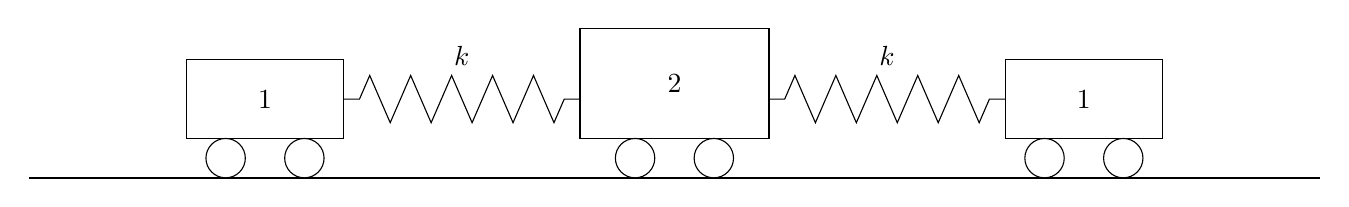
\begin{tikzpicture}
      \draw[thick] (0,0) -- (16.4,0);
      \begin{scope}
        \draw[fill=white] (2,0.5) rectangle node {$1\kg$} (4,1.5);
        \draw[fill=white] (2.5,0.25) circle (0.25);
        \draw[fill=white] (3.5,0.25) circle (0.25);
      \end{scope}
      \begin{scope}[xshift=5.2cm]
        \draw[fill=white] (1.8,0.5) rectangle node {$2\kg$} (4.2,1.9);
        \draw[fill=white] (2.5,0.25) circle (0.25);
        \draw[fill=white] (3.5,0.25) circle (0.25);
      \end{scope}
      \begin{scope}[xshift=10.4cm]
        \draw[fill=white] (2,0.5) rectangle node {$1\kg$} (4,1.5);
        \draw[fill=white] (2.5,0.25) circle (0.25);
        \draw[fill=white] (3.5,0.25) circle (0.25);
      \end{scope}
      \begin{scope}[xshift=4cm]
        \draw (0,1) -- ++(0.2,0) -- ++(0.13,0.3)
        -- ++(0.26,-0.6) -- ++(0.26,0.6)
        -- ++(0.26,-0.6) -- ++(0.26,0.6)
        -- ++(0.26,-0.6) -- ++(0.26,0.6)
        -- ++(0.26,-0.6) -- ++(0.26,0.6)
        -- ++(0.26,-0.6) -- ++(0.13,0.3)
        -- ++(0.2,0);
        \draw (1.5,1.3) node[above] {$k$};
      \end{scope}
      \begin{scope}[xshift=9.4cm]
        \draw (0,1) -- ++(0.2,0) -- ++(0.13,0.3)
        -- ++(0.26,-0.6) -- ++(0.26,0.6)
        -- ++(0.26,-0.6) -- ++(0.26,0.6)
        -- ++(0.26,-0.6) -- ++(0.26,0.6)
        -- ++(0.26,-0.6) -- ++(0.26,0.6)
        -- ++(0.26,-0.6) -- ++(0.13,0.3)
        -- ++(0.2,0);
        \draw (1.5,1.3) node[above] {$k$};
      \end{scope}
    \end{tikzpicture}
  \end{equation*}
  Find and solve the equations of motion of this system.
\end{example}

\begin{solution}
  Let us start by defining appropriate coordinates.  Let $x$ be the
  position of the first car, $y$ the position of the second car, and
  $z$ the position of the third car, measured in meters from left to
  right, relative to each car's natural resting position. The $x$-,
  $y$-, and $z$-axes are shown in the following picture.  All three
  axes are parallel to the train tracks, but they have their origins
  in different places. The coordinates are chosen so that when $x=0$,
  $y=0$, and $z=0$, then all three cars are at rest and both springs
  are in their natural relaxed state.
  \begin{equation*}
    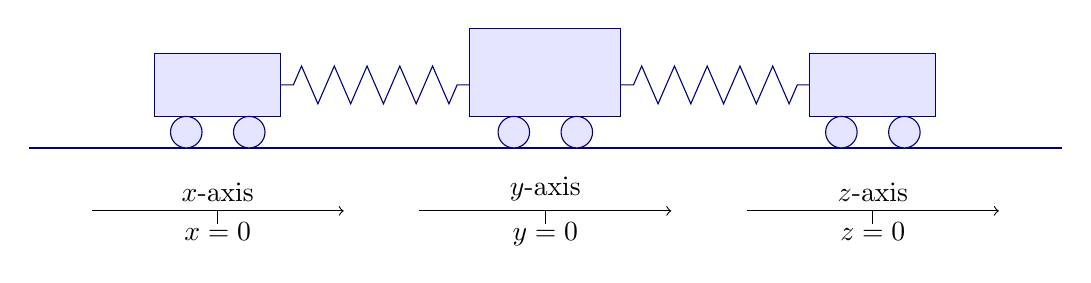
\begin{tikzpicture}[scale=0.8, color=blue!50!black]
      \draw[thick] (0,0) -- (16.4,0);
      \begin{scope}
        \draw[fill=blue!10] (2,0.5) rectangle (4,1.5);
        \draw[fill=blue!10] (2.5,0.25) circle (0.25);
        \draw[fill=blue!10] (3.5,0.25) circle (0.25);
      \end{scope}
      \begin{scope}[xshift=5.2cm]
        \draw[fill=blue!10] (1.8,0.5) rectangle (4.2,1.9);
        \draw[fill=blue!10] (2.5,0.25) circle (0.25);
        \draw[fill=blue!10] (3.5,0.25) circle (0.25);
      \end{scope}
      \begin{scope}[xshift=10.4cm]
        \draw[fill=blue!10] (2,0.5) rectangle (4,1.5);
        \draw[fill=blue!10] (2.5,0.25) circle (0.25);
        \draw[fill=blue!10] (3.5,0.25) circle (0.25);
      \end{scope}
      \begin{scope}[xshift=4cm]
        \draw (0,1) -- ++(0.2,0) -- ++(0.13,0.3)
        -- ++(0.26,-0.6) -- ++(0.26,0.6)
        -- ++(0.26,-0.6) -- ++(0.26,0.6)
        -- ++(0.26,-0.6) -- ++(0.26,0.6)
        -- ++(0.26,-0.6) -- ++(0.26,0.6)
        -- ++(0.26,-0.6) -- ++(0.13,0.3)
        -- ++(0.2,0);
      \end{scope}
      \begin{scope}[xshift=9.4cm]
        \draw (0,1) -- ++(0.2,0) -- ++(0.13,0.3)
        -- ++(0.26,-0.6) -- ++(0.26,0.6)
        -- ++(0.26,-0.6) -- ++(0.26,0.6)
        -- ++(0.26,-0.6) -- ++(0.26,0.6)
        -- ++(0.26,-0.6) -- ++(0.26,0.6)
        -- ++(0.26,-0.6) -- ++(0.13,0.3)
        -- ++(0.2,0);
      \end{scope}
      \begin{scope}[yshift=-1cm, xshift=0cm, color=black]
        \draw[->] (1,0) -- node[above] {$x$-axis} +(4,0);
        \draw (3,0) -- +(0,-0.2) node[below=-4pt] {$x=0$};
      \end{scope}
      \begin{scope}[yshift=-1cm, xshift=5.2cm, color=black]
        \draw[->] (1,0) -- node[above] {$y$-axis} +(4,0);
        \draw (3,0) -- +(0,-0.2) node[below=-4pt] {$y=0$};
      \end{scope}
      \begin{scope}[yshift=-1cm, xshift=10.4cm, color=black]
        \draw[->] (1,0) -- node[above] {$z$-axis} +(4,0);
        \draw (3,0) -- +(0,-0.2) node[below=-4pt] {$z=0$};
      \end{scope}
    \end{tikzpicture}
  \end{equation*}
  Then the extension of the left spring is $y-x$, and therefore the
  left spring's contracting force is
  \begin{equation*}
    F_1 = k(y-x).
  \end{equation*}
  Similarly, the extension of the right spring is $z-y$, and therefore
  its contracting force is
  \begin{equation*}
    F_2 = k(z-y).
  \end{equation*}
  The total force acting on the left car is $F_1$, the total force
  acting on the middle car is $F_2-F_1$, and the total force acting on
  the right car is $-F_2$. By Newton's second law, the acceleration
  of each car is given by $x'' = \frac{F_1}{m_1}$,
  $y'' = \frac{F_2-F_1}{m_2}$, and $z''=\frac{-F_2}{m_3}$. We
  therefore have the following equations of motion:
  \begin{eqnarray*}
    x'' &=& \frac{k}{m_1}(y-x), \\
    y'' &=& \frac{k}{m_2}(x-2y+z), \\
    z'' &=& \frac{k}{m_3}(z-y).
  \end{eqnarray*}
  Let us ignore the physical units and plug in the masses $m_1=1$,
  $m_2=2$, and $m_3=1$ and the spring constant $k=2$. Then the equations
  of motion are:
  \begin{eqnarray*}
    x'' &=& 2(y-x), \\
    y'' &=& x-2y+z, \\
    z'' &=& 2(z-y),
  \end{eqnarray*}
  or equivalently in matrix form:
  \begin{equation*}
    \begin{mymatrix}{c} x'' \\ y'' \\ z'' \end{mymatrix}
    =
    \begin{mymatrix}{rrr}
      -2 & 2 & 0 \\
      1 & -2 & 1 \\
      0 & 2 & -2 \\
    \end{mymatrix}
    \begin{mymatrix}{c} x \\ y \\ z \end{mymatrix}.
  \end{equation*}
  We can also write this as $\vect{v}''=A\vect{v}$, where
  \begin{equation*}
    \vect{v} = \begin{mymatrix}{c} x \\ y \\ z \end{mymatrix}
    \quad\mbox{and}\quad
    A = \begin{mymatrix}{rrr}
      -2 & 2 & 0 \\
      1 & -2 & 1 \\
      0 & 2 & -2 \\
    \end{mymatrix}.
  \end{equation*}
  To solve the equation, we diagonalize the matrix $A$. Using the usual
  method for diagonalization, we find that $A=P^{-1}DP$, where
  \begin{equation*}
    P = \begin{mymatrix}{rrr}
      -1 &  1 & 1 \\
      0  & -1 & 1 \\
      1  &  1 & 1 \\
    \end{mymatrix}
    \quad\mbox{and}\quad
    D = \begin{mymatrix}{rrr}
      -2 &  0 & 0 \\
      0  & -4 & 0 \\
      0  &  0 & 0 \\
    \end{mymatrix}.
  \end{equation*}
  The equation $\vect{v}''=A\vect{v}$ then becomes
  $\vect{v}''=PDP^{-1}\vect{v}$, or equivalently
  $P^{-1}\vect{v}'' = DP^{-1}\vect{v}$. We then diagonalize the
  equation by performing the change of variables
  $\vect{w} = P^{-1}\vect{v}$. The equation becomes
  \begin{equation*}
    \vect{w}'' = D\vect{w}.
  \end{equation*}
  If the components of $\vect{w}$ are called $u$, $v$, and $w$, we can
  write this as
  \begin{equation*}
    \begin{mymatrix}{c} u'' \\ v'' \\ w'' \end{mymatrix}
    =
    \begin{mymatrix}{rrr}
      -2 &  0 & 0 \\
      0  & -4 & 0 \\
      0  &  0 & 0 \\
    \end{mymatrix}
    \begin{mymatrix}{c} u \\ v \\ w \end{mymatrix},
  \end{equation*}
  or equivalently,
  \begin{equation*}
    \begin{array}{c@{~}c@{~}c}
      u'' &=& -2u, \\
      v'' &=& -4v, \\
      w'' &=& 0.   \\
    \end{array}
  \end{equation*}
  Since the variables are now decoupled, we can solve each
  differential equation individually.
  \begin{itemize}
  \item \textbf{Solutions for $\eigenvar=-2$:}
    By Theorem~\ref{thm:differential-equation}, the basic solutions
    for $u'' = -2u$ are
    \begin{equation*}
      u=\sin(\sqrt{2}\,t)
      \quad\mbox{and}\quad
      u=\cos(\sqrt{2}\,t).
    \end{equation*}
    This translates into the following basic solutions for $\vect{w}$:
    \begin{equation*}
      \vect{w}
      = \sin(\sqrt{2}\,t)\begin{mymatrix}{r} 1 \\ 0 \\ 0 \end{mymatrix}
      \quad\mbox{and}\quad
      \vect{w}
      = \cos(\sqrt{2}\,t)\begin{mymatrix}{r} 1 \\ 0 \\ 0 \end{mymatrix}.
    \end{equation*}
    Using $\vect{v} = P\vect{w}$ to change to the original variables,
    we get the basic solutions
    \begin{equation*}
      \vect{v}
      = \sin(\sqrt{2}\,t)\begin{mymatrix}{r} -1 \\ 0 \\ 1 \end{mymatrix}
      \quad\mbox{and}\quad
      \vect{v}
      = \cos(\sqrt{2}\,t)\begin{mymatrix}{r} -1 \\ 0 \\ 1 \end{mymatrix}.
    \end{equation*}
    For example, the first of these basic solutions, written in the
    coordinates $x$, $y$, and $z$, gives
    \begin{equation*}
      \begin{array}{c@{~~}c@{~}l}
        x &=& -\sin(\sqrt{2}\,t), \\
        y &=& ~~~\,0, \\
        z &=& ~~~\sin(\sqrt{2}\,t). \\
      \end{array}
    \end{equation*}
    This corresponds to a periodic oscillation of the train where the
    middle car is stationary, and the left car moves left when the
    right car moves right. Each oscillation takes
    $2\pi/\sqrt{2}\approx 4.4$ seconds.  Here is a ``movie'' showing
    one oscillation:
    \begin{equation*}
      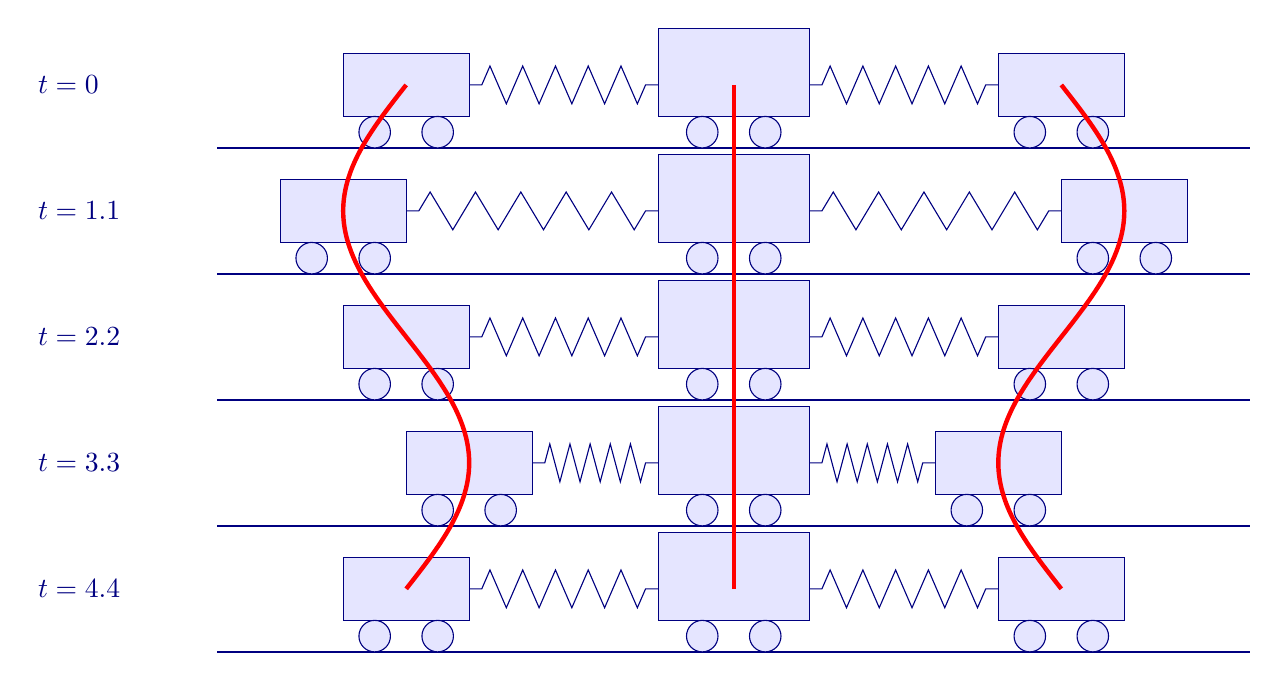
\begin{tikzpicture}[scale=0.8, color=blue!50!black]
        \begin{scope}[yshift=0cm]
          \draw (-3,1) node[right] {$t=0\s$};
          \draw[thick] (0,0) -- (16.4,0);
          \begin{scope}[xshift=0cm]
            \draw[fill=blue!10] (2,0.5) rectangle (4,1.5);
            \draw[fill=blue!10] (2.5,0.25) circle (0.25);
            \draw[fill=blue!10] (3.5,0.25) circle (0.25);
          \end{scope}
          \begin{scope}[xshift=5.2cm]
            \draw[fill=blue!10] (1.8,0.5) rectangle (4.2,1.9);
            \draw[fill=blue!10] (2.5,0.25) circle (0.25);
            \draw[fill=blue!10] (3.5,0.25) circle (0.25);
          \end{scope}
          \begin{scope}[xshift=10.4cm]
            \draw[fill=blue!10] (2,0.5) rectangle (4,1.5);
            \draw[fill=blue!10] (2.5,0.25) circle (0.25);
            \draw[fill=blue!10] (3.5,0.25) circle (0.25);
          \end{scope}
          \begin{scope}[xshift=4cm]
            \draw (0,1) -- ++(0.2,0) -- ++(0.13,0.3)
            -- ++(0.26,-0.6) -- ++(0.26,0.6)
            -- ++(0.26,-0.6) -- ++(0.26,0.6)
            -- ++(0.26,-0.6) -- ++(0.26,0.6)
            -- ++(0.26,-0.6) -- ++(0.26,0.6)
            -- ++(0.26,-0.6) -- ++(0.13,0.3)
            -- ++(0.2,0);
          \end{scope}
          \begin{scope}[xshift=9.4cm]
            \draw (0,1) -- ++(0.2,0) -- ++(0.13,0.3)
            -- ++(0.26,-0.6) -- ++(0.26,0.6)
            -- ++(0.26,-0.6) -- ++(0.26,0.6)
            -- ++(0.26,-0.6) -- ++(0.26,0.6)
            -- ++(0.26,-0.6) -- ++(0.26,0.6)
            -- ++(0.26,-0.6) -- ++(0.13,0.3)
            -- ++(0.2,0);
          \end{scope}
        \end{scope}
        \begin{scope}[yshift=-2cm]
          \draw (-3,1) node[right] {$t=1.1\s$};
          \draw[thick] (0,0) -- (16.4,0);
          \begin{scope}[xshift=-1cm]
            \draw[fill=blue!10] (2,0.5) rectangle (4,1.5);
            \draw[fill=blue!10] (2.5,0.25) circle (0.25);
            \draw[fill=blue!10] (3.5,0.25) circle (0.25);
          \end{scope}
          \begin{scope}[xshift=5.2cm]
            \draw[fill=blue!10] (1.8,0.5) rectangle (4.2,1.9);
            \draw[fill=blue!10] (2.5,0.25) circle (0.25);
            \draw[fill=blue!10] (3.5,0.25) circle (0.25);
          \end{scope}
          \begin{scope}[xshift=11.4cm]
            \draw[fill=blue!10] (2,0.5) rectangle (4,1.5);
            \draw[fill=blue!10] (2.5,0.25) circle (0.25);
            \draw[fill=blue!10] (3.5,0.25) circle (0.25);
          \end{scope}
          \begin{scope}[xshift=3cm]
            \draw (0,1) -- ++(0.2,0) -- ++(0.18,0.3)
            -- ++(0.36,-0.6) -- ++(0.36,0.6)
            -- ++(0.36,-0.6) -- ++(0.36,0.6)
            -- ++(0.36,-0.6) -- ++(0.36,0.6)
            -- ++(0.36,-0.6) -- ++(0.36,0.6)
            -- ++(0.36,-0.6) -- ++(0.18,0.3)
            -- ++(0.2,0);
          \end{scope}
          \begin{scope}[xshift=9.4cm]
            \draw (0,1) -- ++(0.2,0) -- ++(0.18,0.3)
            -- ++(0.36,-0.6) -- ++(0.36,0.6)
            -- ++(0.36,-0.6) -- ++(0.36,0.6)
            -- ++(0.36,-0.6) -- ++(0.36,0.6)
            -- ++(0.36,-0.6) -- ++(0.36,0.6)
            -- ++(0.36,-0.6) -- ++(0.18,0.3)
            -- ++(0.2,0);
          \end{scope}
        \end{scope}
        \begin{scope}[yshift=-4cm]
          \draw (-3,1) node[right] {$t=2.2\s$};
          \draw[thick] (0,0) -- (16.4,0);
          \begin{scope}[xshift=0cm]
            \draw[fill=blue!10] (2,0.5) rectangle (4,1.5);
            \draw[fill=blue!10] (2.5,0.25) circle (0.25);
            \draw[fill=blue!10] (3.5,0.25) circle (0.25);
          \end{scope}
          \begin{scope}[xshift=5.2cm]
            \draw[fill=blue!10] (1.8,0.5) rectangle (4.2,1.9);
            \draw[fill=blue!10] (2.5,0.25) circle (0.25);
            \draw[fill=blue!10] (3.5,0.25) circle (0.25);
          \end{scope}
          \begin{scope}[xshift=10.4cm]
            \draw[fill=blue!10] (2,0.5) rectangle (4,1.5);
            \draw[fill=blue!10] (2.5,0.25) circle (0.25);
            \draw[fill=blue!10] (3.5,0.25) circle (0.25);
          \end{scope}
          \begin{scope}[xshift=4cm]
            \draw (0,1) -- ++(0.2,0) -- ++(0.13,0.3)
            -- ++(0.26,-0.6) -- ++(0.26,0.6)
            -- ++(0.26,-0.6) -- ++(0.26,0.6)
            -- ++(0.26,-0.6) -- ++(0.26,0.6)
            -- ++(0.26,-0.6) -- ++(0.26,0.6)
            -- ++(0.26,-0.6) -- ++(0.13,0.3)
            -- ++(0.2,0);
          \end{scope}
          \begin{scope}[xshift=9.4cm]
            \draw (0,1) -- ++(0.2,0) -- ++(0.13,0.3)
            -- ++(0.26,-0.6) -- ++(0.26,0.6)
            -- ++(0.26,-0.6) -- ++(0.26,0.6)
            -- ++(0.26,-0.6) -- ++(0.26,0.6)
            -- ++(0.26,-0.6) -- ++(0.26,0.6)
            -- ++(0.26,-0.6) -- ++(0.13,0.3)
            -- ++(0.2,0);
          \end{scope}
        \end{scope}
        \begin{scope}[yshift=-6cm]
          \draw (-3,1) node[right] {$t=3.3\s$};
          \draw[thick] (0,0) -- (16.4,0);
          \begin{scope}[xshift=1cm]
            \draw[fill=blue!10] (2,0.5) rectangle (4,1.5);
            \draw[fill=blue!10] (2.5,0.25) circle (0.25);
            \draw[fill=blue!10] (3.5,0.25) circle (0.25);
          \end{scope}
          \begin{scope}[xshift=5.2cm]
            \draw[fill=blue!10] (1.8,0.5) rectangle (4.2,1.9);
            \draw[fill=blue!10] (2.5,0.25) circle (0.25);
            \draw[fill=blue!10] (3.5,0.25) circle (0.25);
          \end{scope}
          \begin{scope}[xshift=9.4cm]
            \draw[fill=blue!10] (2,0.5) rectangle (4,1.5);
            \draw[fill=blue!10] (2.5,0.25) circle (0.25);
            \draw[fill=blue!10] (3.5,0.25) circle (0.25);
          \end{scope}
          \begin{scope}[xshift=5cm]
            \draw (0,1) -- ++(0.2,0) -- ++(0.08,0.3)
            -- ++(0.16,-0.6) -- ++(0.16,0.6)
            -- ++(0.16,-0.6) -- ++(0.16,0.6)
            -- ++(0.16,-0.6) -- ++(0.16,0.6)
            -- ++(0.16,-0.6) -- ++(0.16,0.6)
            -- ++(0.16,-0.6) -- ++(0.08,0.3)
            -- ++(0.2,0);
          \end{scope}
          \begin{scope}[xshift=9.4cm]
            \draw (0,1) -- ++(0.2,0) -- ++(0.08,0.3)
            -- ++(0.16,-0.6) -- ++(0.16,0.6)
            -- ++(0.16,-0.6) -- ++(0.16,0.6)
            -- ++(0.16,-0.6) -- ++(0.16,0.6)
            -- ++(0.16,-0.6) -- ++(0.16,0.6)
            -- ++(0.16,-0.6) -- ++(0.08,0.3)
            -- ++(0.2,0);
          \end{scope}
        \end{scope}
        \begin{scope}[yshift=-8cm]
          \draw (-3,1) node[right] {$t=4.4\s$};
          \draw[thick] (0,0) -- (16.4,0);
          \begin{scope}[xshift=0cm]
            \draw[fill=blue!10] (2,0.5) rectangle (4,1.5);
            \draw[fill=blue!10] (2.5,0.25) circle (0.25);
            \draw[fill=blue!10] (3.5,0.25) circle (0.25);
          \end{scope}
          \begin{scope}[xshift=5.2cm]
            \draw[fill=blue!10] (1.8,0.5) rectangle (4.2,1.9);
            \draw[fill=blue!10] (2.5,0.25) circle (0.25);
            \draw[fill=blue!10] (3.5,0.25) circle (0.25);
          \end{scope}
          \begin{scope}[xshift=10.4cm]
            \draw[fill=blue!10] (2,0.5) rectangle (4,1.5);
            \draw[fill=blue!10] (2.5,0.25) circle (0.25);
            \draw[fill=blue!10] (3.5,0.25) circle (0.25);
          \end{scope}
          \begin{scope}[xshift=4cm]
            \draw (0,1) -- ++(0.2,0) -- ++(0.13,0.3)
            -- ++(0.26,-0.6) -- ++(0.26,0.6)
            -- ++(0.26,-0.6) -- ++(0.26,0.6)
            -- ++(0.26,-0.6) -- ++(0.26,0.6)
            -- ++(0.26,-0.6) -- ++(0.26,0.6)
            -- ++(0.26,-0.6) -- ++(0.13,0.3)
            -- ++(0.2,0);
          \end{scope}
          \begin{scope}[xshift=9.4cm]
            \draw (0,1) -- ++(0.2,0) -- ++(0.13,0.3)
            -- ++(0.26,-0.6) -- ++(0.26,0.6)
            -- ++(0.26,-0.6) -- ++(0.26,0.6)
            -- ++(0.26,-0.6) -- ++(0.26,0.6)
            -- ++(0.26,-0.6) -- ++(0.26,0.6)
            -- ++(0.26,-0.6) -- ++(0.13,0.3)
            -- ++(0.2,0);
          \end{scope}
        \end{scope}
        \begin{scope}[xshift=3cm,yshift=1cm,rotate=-90]
          \draw[ultra thick,red] (0,0) sin (2,-1) cos (4,0) sin (6,1) cos (8,0);
        \end{scope}
        \begin{scope}[xshift=8.2cm,yshift=1cm,rotate=-90]
          \draw[ultra thick,red] (0,0) sin (2,0) cos (4,0) sin (6,0) cos (8,0);
        \end{scope}
        \begin{scope}[xshift=13.4cm,yshift=1cm,rotate=-90]
          \draw[ultra thick,red] (0,0) sin (2,1) cos (4,0) sin (6,-1) cos (8,0);
        \end{scope}
      \end{tikzpicture}
    \end{equation*}
    The other basic solution, with $\cos$ instead of $\sin$, is the
    same motion, just starting at a different offset in time. Note how
    the eigenvector of $A$,
    \begin{equation*}
      \begin{mymatrix}{r} -1 \\ 0 \\ 1 \end{mymatrix},
    \end{equation*}
    describes the relative motion of the three cars, i.e., the first
    and last cars are moving in opposite directions, whereas the
    middle car is stationary. The corresponding eigenvalue
    $\eigenvar=-2$ determines the frequency. The frequency, which is
    $\sqrt{2}/2\pi$ oscillations per second, is also called an
    \textbf{eigenfrequency}%
    \index{eigenfrequency}%
    \index{differential equation!eigenfrequency} or \textbf{resonance
      frequency}%
    \index{resonance!frequency}%
    \index{differential equation!resonance frequency}%
    \index{frequency!resonance} of the system.
  \item \textbf{Solutions for $\eigenvar=-4$:}
    By Theorem~\ref{thm:differential-equation}, the basic solutions
    for $v'' = -4v$ are
    \begin{equation*}
      v=\sin(2t)
      \quad\mbox{and}\quad
      v=\cos(2t).
    \end{equation*}
    This translates into the following basic solutions for $\vect{w}$:
    \begin{equation*}
      \vect{w}
      = \sin(2t)\begin{mymatrix}{r} 0 \\ 1 \\ 0 \end{mymatrix}
      \quad\mbox{and}\quad
      \vect{w}
      = \cos(2t)\begin{mymatrix}{r} 0 \\ 1 \\ 0 \end{mymatrix}.
    \end{equation*}
    We change this to the original variables using $\vect{v} =
    P\vect{w}$, and get the basic solutions
    \begin{equation*}
      \vect{v}
      = \sin(2t)\begin{mymatrix}{r} 1 \\ -1 \\ 1 \end{mymatrix}
      \quad\mbox{and}\quad
      \vect{v}
      = \cos(2t)\begin{mymatrix}{r} 1 \\ -1 \\ 1 \end{mymatrix}.
    \end{equation*}
    Writing the first of these basic solutions in the coordinates $x$,
    $y$, and $z$, we get
    \begin{equation*}
      \begin{array}{c@{~~}c@{~}l}
        x &=& ~~~\sin(2t), \\
        y &=& -\sin(2t), \\
        z &=& ~~~\sin(2t). \\
      \end{array}
    \end{equation*}
    This corresponds to a periodic oscillation of the train where the
    outer cars move right at the same time that the middle car moves
    left. Each oscillation takes
    $2\pi/2\approx 3.14$ seconds. Here is a ``movie'' of the motion:
    \begin{equation*}
      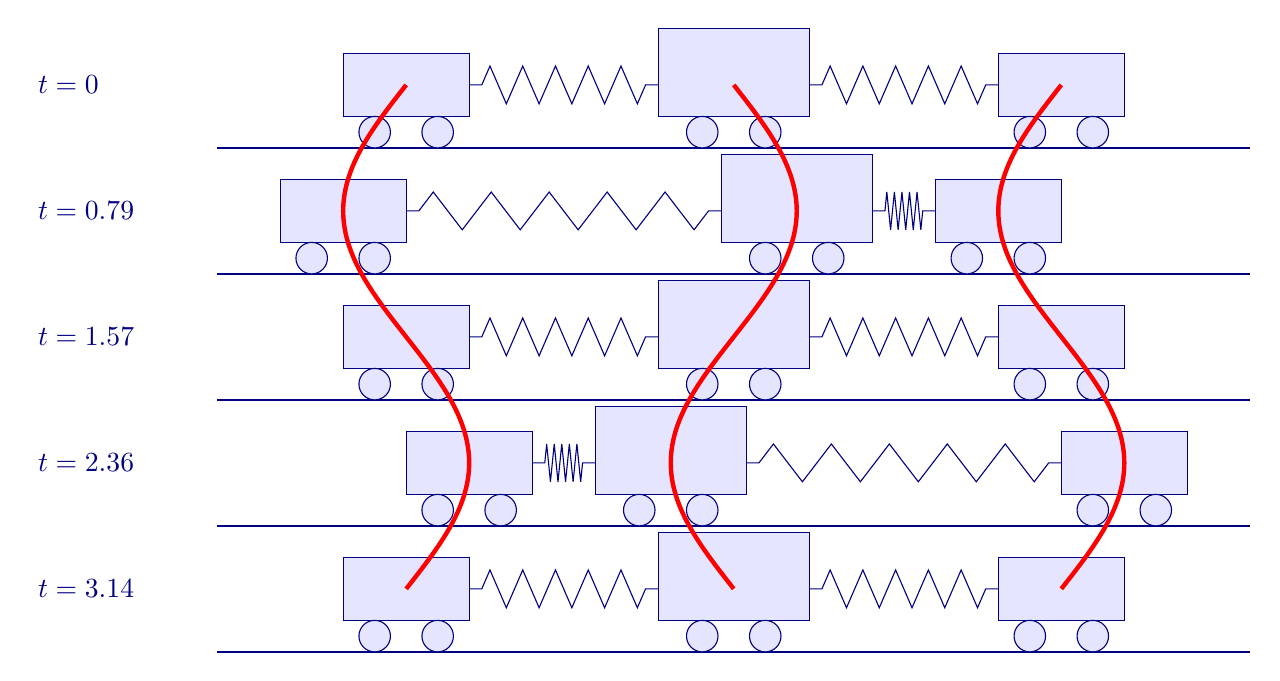
\begin{tikzpicture}[scale=0.8, color=blue!50!black]
        \begin{scope}[yshift=0cm]
          \draw (-3,1) node[right] {$t=0\s$};
          \draw[thick] (0,0) -- (16.4,0);
          \begin{scope}[xshift=0cm]
            \draw[fill=blue!10] (2,0.5) rectangle (4,1.5);
            \draw[fill=blue!10] (2.5,0.25) circle (0.25);
            \draw[fill=blue!10] (3.5,0.25) circle (0.25);
          \end{scope}
          \begin{scope}[xshift=5.2cm]
            \draw[fill=blue!10] (1.8,0.5) rectangle (4.2,1.9);
            \draw[fill=blue!10] (2.5,0.25) circle (0.25);
            \draw[fill=blue!10] (3.5,0.25) circle (0.25);
          \end{scope}
          \begin{scope}[xshift=10.4cm]
            \draw[fill=blue!10] (2,0.5) rectangle (4,1.5);
            \draw[fill=blue!10] (2.5,0.25) circle (0.25);
            \draw[fill=blue!10] (3.5,0.25) circle (0.25);
          \end{scope}
          \begin{scope}[xshift=4cm]
            \draw (0,1) -- ++(0.2,0) -- ++(0.13,0.3)
            -- ++(0.26,-0.6) -- ++(0.26,0.6)
            -- ++(0.26,-0.6) -- ++(0.26,0.6)
            -- ++(0.26,-0.6) -- ++(0.26,0.6)
            -- ++(0.26,-0.6) -- ++(0.26,0.6)
            -- ++(0.26,-0.6) -- ++(0.13,0.3)
            -- ++(0.2,0);
          \end{scope}
          \begin{scope}[xshift=9.4cm]
            \draw (0,1) -- ++(0.2,0) -- ++(0.13,0.3)
            -- ++(0.26,-0.6) -- ++(0.26,0.6)
            -- ++(0.26,-0.6) -- ++(0.26,0.6)
            -- ++(0.26,-0.6) -- ++(0.26,0.6)
            -- ++(0.26,-0.6) -- ++(0.26,0.6)
            -- ++(0.26,-0.6) -- ++(0.13,0.3)
            -- ++(0.2,0);
          \end{scope}
        \end{scope}
        \begin{scope}[yshift=-2cm]
          \draw (-3,1) node[right] {$t=0.79\s$};
          \draw[thick] (0,0) -- (16.4,0);
          \begin{scope}[xshift=-1cm]
            \draw[fill=blue!10] (2,0.5) rectangle (4,1.5);
            \draw[fill=blue!10] (2.5,0.25) circle (0.25);
            \draw[fill=blue!10] (3.5,0.25) circle (0.25);
          \end{scope}
          \begin{scope}[xshift=6.2cm]
            \draw[fill=blue!10] (1.8,0.5) rectangle (4.2,1.9);
            \draw[fill=blue!10] (2.5,0.25) circle (0.25);
            \draw[fill=blue!10] (3.5,0.25) circle (0.25);
          \end{scope}
          \begin{scope}[xshift=9.4cm]
            \draw[fill=blue!10] (2,0.5) rectangle (4,1.5);
            \draw[fill=blue!10] (2.5,0.25) circle (0.25);
            \draw[fill=blue!10] (3.5,0.25) circle (0.25);
          \end{scope}
          \begin{scope}[xshift=3cm]
            \draw (0,1) -- ++(0.2,0) -- ++(0.23,0.3)
            -- ++(0.46,-0.6) -- ++(0.46,0.6)
            -- ++(0.46,-0.6) -- ++(0.46,0.6)
            -- ++(0.46,-0.6) -- ++(0.46,0.6)
            -- ++(0.46,-0.6) -- ++(0.46,0.6)
            -- ++(0.46,-0.6) -- ++(0.23,0.3)
            -- ++(0.2,0);
          \end{scope}
          \begin{scope}[xshift=10.4cm]
            \draw (0,1) -- ++(0.2,0) -- ++(0.03,0.3)
            -- ++(0.06,-0.6) -- ++(0.06,0.6)
            -- ++(0.06,-0.6) -- ++(0.06,0.6)
            -- ++(0.06,-0.6) -- ++(0.06,0.6)
            -- ++(0.06,-0.6) -- ++(0.06,0.6)
            -- ++(0.06,-0.6) -- ++(0.03,0.3)
            -- ++(0.2,0);
          \end{scope}
        \end{scope}
        \begin{scope}[yshift=-4cm]
          \draw (-3,1) node[right] {$t=1.57\s$};
          \draw[thick] (0,0) -- (16.4,0);
          \begin{scope}[xshift=0cm]
            \draw[fill=blue!10] (2,0.5) rectangle (4,1.5);
            \draw[fill=blue!10] (2.5,0.25) circle (0.25);
            \draw[fill=blue!10] (3.5,0.25) circle (0.25);
          \end{scope}
          \begin{scope}[xshift=5.2cm]
            \draw[fill=blue!10] (1.8,0.5) rectangle (4.2,1.9);
            \draw[fill=blue!10] (2.5,0.25) circle (0.25);
            \draw[fill=blue!10] (3.5,0.25) circle (0.25);
          \end{scope}
          \begin{scope}[xshift=10.4cm]
            \draw[fill=blue!10] (2,0.5) rectangle (4,1.5);
            \draw[fill=blue!10] (2.5,0.25) circle (0.25);
            \draw[fill=blue!10] (3.5,0.25) circle (0.25);
          \end{scope}
          \begin{scope}[xshift=4cm]
            \draw (0,1) -- ++(0.2,0) -- ++(0.13,0.3)
            -- ++(0.26,-0.6) -- ++(0.26,0.6)
            -- ++(0.26,-0.6) -- ++(0.26,0.6)
            -- ++(0.26,-0.6) -- ++(0.26,0.6)
            -- ++(0.26,-0.6) -- ++(0.26,0.6)
            -- ++(0.26,-0.6) -- ++(0.13,0.3)
            -- ++(0.2,0);
          \end{scope}
          \begin{scope}[xshift=9.4cm]
            \draw (0,1) -- ++(0.2,0) -- ++(0.13,0.3)
            -- ++(0.26,-0.6) -- ++(0.26,0.6)
            -- ++(0.26,-0.6) -- ++(0.26,0.6)
            -- ++(0.26,-0.6) -- ++(0.26,0.6)
            -- ++(0.26,-0.6) -- ++(0.26,0.6)
            -- ++(0.26,-0.6) -- ++(0.13,0.3)
            -- ++(0.2,0);
          \end{scope}
        \end{scope}
        \begin{scope}[yshift=-6cm]
          \draw (-3,1) node[right] {$t=2.36\s$};
          \draw[thick] (0,0) -- (16.4,0);
          \begin{scope}[xshift=1cm]
            \draw[fill=blue!10] (2,0.5) rectangle (4,1.5);
            \draw[fill=blue!10] (2.5,0.25) circle (0.25);
            \draw[fill=blue!10] (3.5,0.25) circle (0.25);
          \end{scope}
          \begin{scope}[xshift=4.2cm]
            \draw[fill=blue!10] (1.8,0.5) rectangle (4.2,1.9);
            \draw[fill=blue!10] (2.5,0.25) circle (0.25);
            \draw[fill=blue!10] (3.5,0.25) circle (0.25);
          \end{scope}
          \begin{scope}[xshift=11.4cm]
            \draw[fill=blue!10] (2,0.5) rectangle (4,1.5);
            \draw[fill=blue!10] (2.5,0.25) circle (0.25);
            \draw[fill=blue!10] (3.5,0.25) circle (0.25);
          \end{scope}
          \begin{scope}[xshift=5cm]
            \draw (0,1) -- ++(0.2,0) -- ++(0.03,0.3)
            -- ++(0.06,-0.6) -- ++(0.06,0.6)
            -- ++(0.06,-0.6) -- ++(0.06,0.6)
            -- ++(0.06,-0.6) -- ++(0.06,0.6)
            -- ++(0.06,-0.6) -- ++(0.06,0.6)
            -- ++(0.06,-0.6) -- ++(0.03,0.3)
            -- ++(0.2,0);
          \end{scope}
          \begin{scope}[xshift=8.4cm]
            \draw (0,1) -- ++(0.2,0) -- ++(0.23,0.3)
            -- ++(0.46,-0.6) -- ++(0.46,0.6)
            -- ++(0.46,-0.6) -- ++(0.46,0.6)
            -- ++(0.46,-0.6) -- ++(0.46,0.6)
            -- ++(0.46,-0.6) -- ++(0.46,0.6)
            -- ++(0.46,-0.6) -- ++(0.23,0.3)
            -- ++(0.2,0);
          \end{scope}
        \end{scope}
        \begin{scope}[yshift=-8cm]
          \draw (-3,1) node[right] {$t=3.14\s$};
          \draw[thick] (0,0) -- (16.4,0);
          \begin{scope}[xshift=0cm]
            \draw[fill=blue!10] (2,0.5) rectangle (4,1.5);
            \draw[fill=blue!10] (2.5,0.25) circle (0.25);
            \draw[fill=blue!10] (3.5,0.25) circle (0.25);
          \end{scope}
          \begin{scope}[xshift=5.2cm]
            \draw[fill=blue!10] (1.8,0.5) rectangle (4.2,1.9);
            \draw[fill=blue!10] (2.5,0.25) circle (0.25);
            \draw[fill=blue!10] (3.5,0.25) circle (0.25);
          \end{scope}
          \begin{scope}[xshift=10.4cm]
            \draw[fill=blue!10] (2,0.5) rectangle (4,1.5);
            \draw[fill=blue!10] (2.5,0.25) circle (0.25);
            \draw[fill=blue!10] (3.5,0.25) circle (0.25);
          \end{scope}
          \begin{scope}[xshift=4cm]
            \draw (0,1) -- ++(0.2,0) -- ++(0.13,0.3)
            -- ++(0.26,-0.6) -- ++(0.26,0.6)
            -- ++(0.26,-0.6) -- ++(0.26,0.6)
            -- ++(0.26,-0.6) -- ++(0.26,0.6)
            -- ++(0.26,-0.6) -- ++(0.26,0.6)
            -- ++(0.26,-0.6) -- ++(0.13,0.3)
            -- ++(0.2,0);
          \end{scope}
          \begin{scope}[xshift=9.4cm]
            \draw (0,1) -- ++(0.2,0) -- ++(0.13,0.3)
            -- ++(0.26,-0.6) -- ++(0.26,0.6)
            -- ++(0.26,-0.6) -- ++(0.26,0.6)
            -- ++(0.26,-0.6) -- ++(0.26,0.6)
            -- ++(0.26,-0.6) -- ++(0.26,0.6)
            -- ++(0.26,-0.6) -- ++(0.13,0.3)
            -- ++(0.2,0);
          \end{scope}
        \end{scope}
        \begin{scope}[xshift=3cm,yshift=1cm,rotate=-90]
          \draw[ultra thick,red] (0,0) sin (2,-1) cos (4,0) sin (6,1) cos (8,0);
        \end{scope}
        \begin{scope}[xshift=8.2cm,yshift=1cm,rotate=-90]
          \draw[ultra thick,red] (0,0) sin (2,1) cos (4,0) sin (6,-1) cos (8,0);
        \end{scope}
        \begin{scope}[xshift=13.4cm,yshift=1cm,rotate=-90]
          \draw[ultra thick,red] (0,0) sin (2,-1) cos (4,0) sin (6,1) cos (8,0);
        \end{scope}
      \end{tikzpicture}
    \end{equation*}
    As before, the other basic solution, using $\cos$ instead of
    $\sin$, is the same motion, but shifted in time. Also, the
    eigenvector
    \begin{equation*}
      \begin{mymatrix}{r} 1 \\ -1 \\ 1 \end{mymatrix}
    \end{equation*}
    describes the relative motion of the three cars; here the first
    and last car move in the same direction while the middle car moves
    in the opposite direction. The eigenfrequency of this oscillation,
    at $2/2\pi$ oscillations per second, is slightly higher than the
    first one, due to the larger magnitude of the eigenvalue
    $\eigenvar=-4$.
  \item \textbf{Solutions for $\eigenvar=0$:} The last eigenvalue is
    zero. By Theorem~\ref{thm:differential-equation}, the general
    solution of $w'' = 0$ is
    \begin{equation*}
      w = a+bt,
    \end{equation*}
    where $a$ and $b$ are arbitrary constants. This translates into
    the following solution for $\vect{w}$:
    \begin{equation*}
      \vect{w}
      = (a+bt)\begin{mymatrix}{r} 0 \\ 0 \\ 1 \end{mymatrix},
    \end{equation*}
    and by the change of variables $\vect{v} = P\vect{w}$, we get
    \begin{equation*}
      \vect{v}
      = (a+bt)\begin{mymatrix}{r} 1 \\ 1 \\ 1 \end{mymatrix}.
    \end{equation*}
    Writing this in terms of the coordinates $x$, $y$, and $z$, we get
    \begin{equation*}
      \begin{array}{c@{~~}c@{~}l}
        x &=& a+bt, \\
        y &=& a+bt, \\
        z &=& a+bt. \\
      \end{array}
    \end{equation*}
    This simply describes a linear motion: the three cars are moving
    down the track at constant speed $b$ from some initial starting
    position $a$.
    \begin{equation*}
      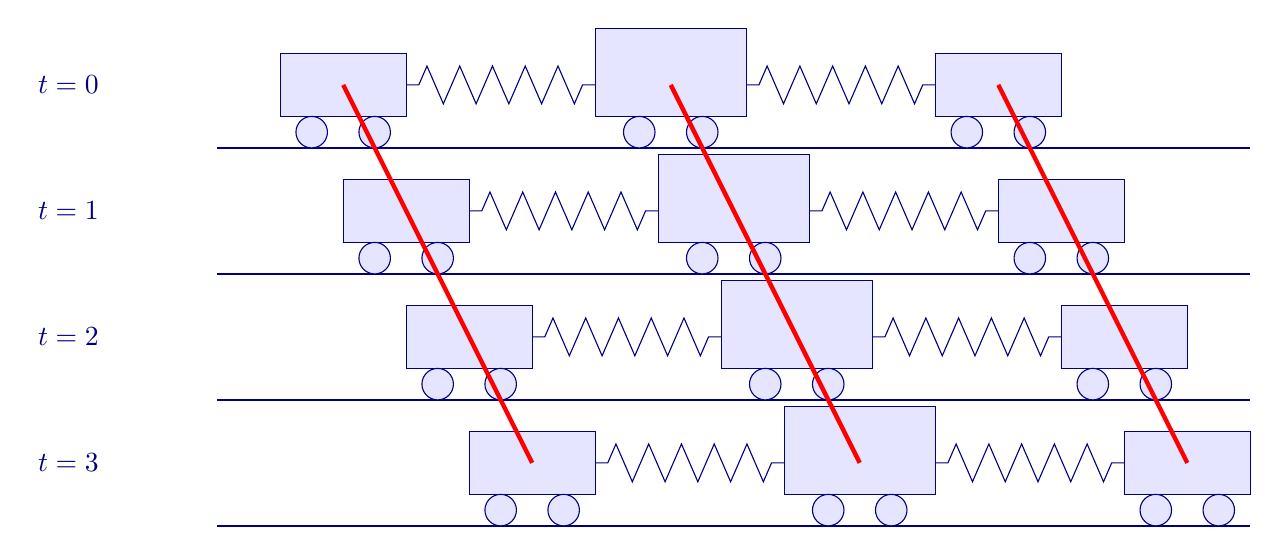
\begin{tikzpicture}[scale=0.8, color=blue!50!black]
        \begin{scope}[yshift=0cm]
          \draw (-3,1) node[right] {$t=0\s$};
          \draw[thick] (0,0) -- (16.4,0);
          \begin{scope}[xshift=-1cm]
            \draw[fill=blue!10] (2,0.5) rectangle (4,1.5);
            \draw[fill=blue!10] (2.5,0.25) circle (0.25);
            \draw[fill=blue!10] (3.5,0.25) circle (0.25);
          \end{scope}
          \begin{scope}[xshift=4.2cm]
            \draw[fill=blue!10] (1.8,0.5) rectangle (4.2,1.9);
            \draw[fill=blue!10] (2.5,0.25) circle (0.25);
            \draw[fill=blue!10] (3.5,0.25) circle (0.25);
          \end{scope}
          \begin{scope}[xshift=9.4cm]
            \draw[fill=blue!10] (2,0.5) rectangle (4,1.5);
            \draw[fill=blue!10] (2.5,0.25) circle (0.25);
            \draw[fill=blue!10] (3.5,0.25) circle (0.25);
          \end{scope}
          \begin{scope}[xshift=3cm]
            \draw (0,1) -- ++(0.2,0) -- ++(0.13,0.3)
            -- ++(0.26,-0.6) -- ++(0.26,0.6)
            -- ++(0.26,-0.6) -- ++(0.26,0.6)
            -- ++(0.26,-0.6) -- ++(0.26,0.6)
            -- ++(0.26,-0.6) -- ++(0.26,0.6)
            -- ++(0.26,-0.6) -- ++(0.13,0.3)
            -- ++(0.2,0);
          \end{scope}
          \begin{scope}[xshift=8.4cm]
            \draw (0,1) -- ++(0.2,0) -- ++(0.13,0.3)
            -- ++(0.26,-0.6) -- ++(0.26,0.6)
            -- ++(0.26,-0.6) -- ++(0.26,0.6)
            -- ++(0.26,-0.6) -- ++(0.26,0.6)
            -- ++(0.26,-0.6) -- ++(0.26,0.6)
            -- ++(0.26,-0.6) -- ++(0.13,0.3)
            -- ++(0.2,0);
          \end{scope}
        \end{scope}
        \begin{scope}[yshift=-2cm]
          \draw (-3,1) node[right] {$t=1\s$};
          \draw[thick] (0,0) -- (16.4,0);
          \begin{scope}[xshift=0cm]
            \draw[fill=blue!10] (2,0.5) rectangle (4,1.5);
            \draw[fill=blue!10] (2.5,0.25) circle (0.25);
            \draw[fill=blue!10] (3.5,0.25) circle (0.25);
          \end{scope}
          \begin{scope}[xshift=5.2cm]
            \draw[fill=blue!10] (1.8,0.5) rectangle (4.2,1.9);
            \draw[fill=blue!10] (2.5,0.25) circle (0.25);
            \draw[fill=blue!10] (3.5,0.25) circle (0.25);
          \end{scope}
          \begin{scope}[xshift=10.4cm]
            \draw[fill=blue!10] (2,0.5) rectangle (4,1.5);
            \draw[fill=blue!10] (2.5,0.25) circle (0.25);
            \draw[fill=blue!10] (3.5,0.25) circle (0.25);
          \end{scope}
          \begin{scope}[xshift=4cm]
            \draw (0,1) -- ++(0.2,0) -- ++(0.13,0.3)
            -- ++(0.26,-0.6) -- ++(0.26,0.6)
            -- ++(0.26,-0.6) -- ++(0.26,0.6)
            -- ++(0.26,-0.6) -- ++(0.26,0.6)
            -- ++(0.26,-0.6) -- ++(0.26,0.6)
            -- ++(0.26,-0.6) -- ++(0.13,0.3)
            -- ++(0.2,0);
          \end{scope}
          \begin{scope}[xshift=9.4cm]
            \draw (0,1) -- ++(0.2,0) -- ++(0.13,0.3)
            -- ++(0.26,-0.6) -- ++(0.26,0.6)
            -- ++(0.26,-0.6) -- ++(0.26,0.6)
            -- ++(0.26,-0.6) -- ++(0.26,0.6)
            -- ++(0.26,-0.6) -- ++(0.26,0.6)
            -- ++(0.26,-0.6) -- ++(0.13,0.3)
            -- ++(0.2,0);
          \end{scope}
        \end{scope}
        \begin{scope}[yshift=-4cm]
          \draw (-3,1) node[right] {$t=2\s$};
          \draw[thick] (0,0) -- (16.4,0);
          \begin{scope}[xshift=1cm]
            \draw[fill=blue!10] (2,0.5) rectangle (4,1.5);
            \draw[fill=blue!10] (2.5,0.25) circle (0.25);
            \draw[fill=blue!10] (3.5,0.25) circle (0.25);
          \end{scope}
          \begin{scope}[xshift=6.2cm]
            \draw[fill=blue!10] (1.8,0.5) rectangle (4.2,1.9);
            \draw[fill=blue!10] (2.5,0.25) circle (0.25);
            \draw[fill=blue!10] (3.5,0.25) circle (0.25);
          \end{scope}
          \begin{scope}[xshift=11.4cm]
            \draw[fill=blue!10] (2,0.5) rectangle (4,1.5);
            \draw[fill=blue!10] (2.5,0.25) circle (0.25);
            \draw[fill=blue!10] (3.5,0.25) circle (0.25);
          \end{scope}
          \begin{scope}[xshift=5cm]
            \draw (0,1) -- ++(0.2,0) -- ++(0.13,0.3)
            -- ++(0.26,-0.6) -- ++(0.26,0.6)
            -- ++(0.26,-0.6) -- ++(0.26,0.6)
            -- ++(0.26,-0.6) -- ++(0.26,0.6)
            -- ++(0.26,-0.6) -- ++(0.26,0.6)
            -- ++(0.26,-0.6) -- ++(0.13,0.3)
            -- ++(0.2,0);
          \end{scope}
          \begin{scope}[xshift=10.4cm]
            \draw (0,1) -- ++(0.2,0) -- ++(0.13,0.3)
            -- ++(0.26,-0.6) -- ++(0.26,0.6)
            -- ++(0.26,-0.6) -- ++(0.26,0.6)
            -- ++(0.26,-0.6) -- ++(0.26,0.6)
            -- ++(0.26,-0.6) -- ++(0.26,0.6)
            -- ++(0.26,-0.6) -- ++(0.13,0.3)
            -- ++(0.2,0);
          \end{scope}
        \end{scope}
        \begin{scope}[yshift=-6cm]
          \draw (-3,1) node[right] {$t=3\s$};
          \draw[thick] (0,0) -- (16.4,0);
          \begin{scope}[xshift=2cm]
            \draw[fill=blue!10] (2,0.5) rectangle (4,1.5);
            \draw[fill=blue!10] (2.5,0.25) circle (0.25);
            \draw[fill=blue!10] (3.5,0.25) circle (0.25);
          \end{scope}
          \begin{scope}[xshift=7.2cm]
            \draw[fill=blue!10] (1.8,0.5) rectangle (4.2,1.9);
            \draw[fill=blue!10] (2.5,0.25) circle (0.25);
            \draw[fill=blue!10] (3.5,0.25) circle (0.25);
          \end{scope}
          \begin{scope}[xshift=12.4cm]
            \draw[fill=blue!10] (2,0.5) rectangle (4,1.5);
            \draw[fill=blue!10] (2.5,0.25) circle (0.25);
            \draw[fill=blue!10] (3.5,0.25) circle (0.25);
          \end{scope}
          \begin{scope}[xshift=6cm]
            \draw (0,1) -- ++(0.2,0) -- ++(0.13,0.3)
            -- ++(0.26,-0.6) -- ++(0.26,0.6)
            -- ++(0.26,-0.6) -- ++(0.26,0.6)
            -- ++(0.26,-0.6) -- ++(0.26,0.6)
            -- ++(0.26,-0.6) -- ++(0.26,0.6)
            -- ++(0.26,-0.6) -- ++(0.13,0.3)
            -- ++(0.2,0);
          \end{scope}
          \begin{scope}[xshift=11.4cm]
            \draw (0,1) -- ++(0.2,0) -- ++(0.13,0.3)
            -- ++(0.26,-0.6) -- ++(0.26,0.6)
            -- ++(0.26,-0.6) -- ++(0.26,0.6)
            -- ++(0.26,-0.6) -- ++(0.26,0.6)
            -- ++(0.26,-0.6) -- ++(0.26,0.6)
            -- ++(0.26,-0.6) -- ++(0.13,0.3)
            -- ++(0.2,0);
          \end{scope}
        \end{scope}
        \begin{scope}[xshift=3cm,yshift=1cm,rotate=-90]
          \draw[ultra thick, red] (0,-1) -- (6,2);
        \end{scope}
        \begin{scope}[xshift=8.2cm,yshift=1cm,rotate=-90]
          \draw[ultra thick, red] (0,-1) -- (6,2);
        \end{scope}
        \begin{scope}[xshift=13.4cm,yshift=1cm,rotate=-90]
          \draw[ultra thick, red] (0,-1) -- (6,2);
        \end{scope}
      \end{tikzpicture}
    \end{equation*}
    As before, the eigenvector
    \begin{equation*}
      \begin{mymatrix}{r} 1 \\ 1 \\ 1 \end{mymatrix}
    \end{equation*}
    describes the relative motion of the three cars (in this case all
    moving in the same direction). The eigenvalue $\eigenvar=0$
    indicates linear motion.
  \end{itemize}
  What we have described here are the {\em basic} solutions of the
  system. The solutions corresponding to each of the eigenvalues are
  also called \textbf{modes}%
  \index{mode of resonance}%
  \index{resonance!mode}%
  \index{differential equation!mode} of the system. Thus, the train
  has three modes, each corresponding to a particular eigenvalue of
  the matrix $A$. In the first mode, the middle car is stationary and
  the other two cars oscillate in opposite directions.  In the second
  mode, the middle car oscillates in the opposite direction of the two
  outer cars. The third mode is a linear movement along the track.

  As always, the general solution is a linear combination of basic
  solutions; for example, the cars might be oscillating in both the
  first and second modes at their respective frequencies, while also
  moving down the tracks.
\end{solution}
